\subsection{Case study}
We collaborated with the domain experts to demonstrate the effectiveness of $\DQV$ by analyzing several real world cases which are slower than our exception.

\subsubsection{Identify the hardware bottleneck}
The first case is executed on a cluster with 5 nodes and run around 623 seconds. The execution plan is shown as the Figure~\ref{fig:teaser}(A).

When exploring the execution with $\DQV$, we find that in the progress view, it is obvious Map1(Figure~\ref{fig:teaser}(B1)) significantly run longer than the duration of other vertices. On the other side, the Reducer2, a subsequent vertex of Map1, finished in a very short time after Map1 is finished. Reducer is followed by a sequence of short reduce vertices(shown as Figure~\ref{fig:teaser}(B3)) which are quickly executed after that. 
From this pattern, we guess the bottleneck should be related Map1, several abnormal tasks may lead to the long execution time of Map1. We hover the mouse on it to highlight the associated tasks as blue color in the Distribution View.
In the summary distribution view, we can see there are two task groups which are distributed far away from each other (shown as Figure~\ref{fig:teaser}(C5, C6)). 
By checking the blue-colored tasks on the machine views through cross-view linking, we find the tasks at the left top corner are dispatched on the machine dbg14, dbg16, dbg19 and dbg20. But the tasks on the right bottom corner are only executed on machine dbg18. Moreover, it seems that dbg18 only executes very few tasks in this case. 
We further check the cluster and notice that something wrong with the network of dbg18, thus the tasks assigned to it are delayed and executed very late, leading to the overall long duration of the query execution. In the exploration of summary view, we can find the these tasks of Map1 provides the data to several tasks of Reducer2, shown as the Figure~\ref{fig:teaser}(C1), which also verifies our assumption. 

In addition to Map1, we notice another vertex Map24 also have a very long duration. When we click to mark the tasks of Map24 (these tasks are colored as purple), we find that none of them are executed on dbg18. So we guess dbg18 is not the only reason results in the slow query. At the same time, there is one task run with a very long time (shown as Figure~\ref{fig:teaser}(C2)) on the machine dbg19. Moreover, the dbg19 executes far fewer tasks than the machine dbg14, dbg16 and dbg20, but these tasks tends to have longer duration. By exploring the performance view, we find the CPU usage view of dbg19 has large piece of red color region, indicating the the CPU is more busy than the other machines(shown as Figure~\ref{fig:teaser}(C3)). We further explore the system log and find there are several computing-bounded programs are executed on dbg19 at the same time which takes the computing resource thus making these query tasks very slow.

\begin{figure}[t]
	\centering
	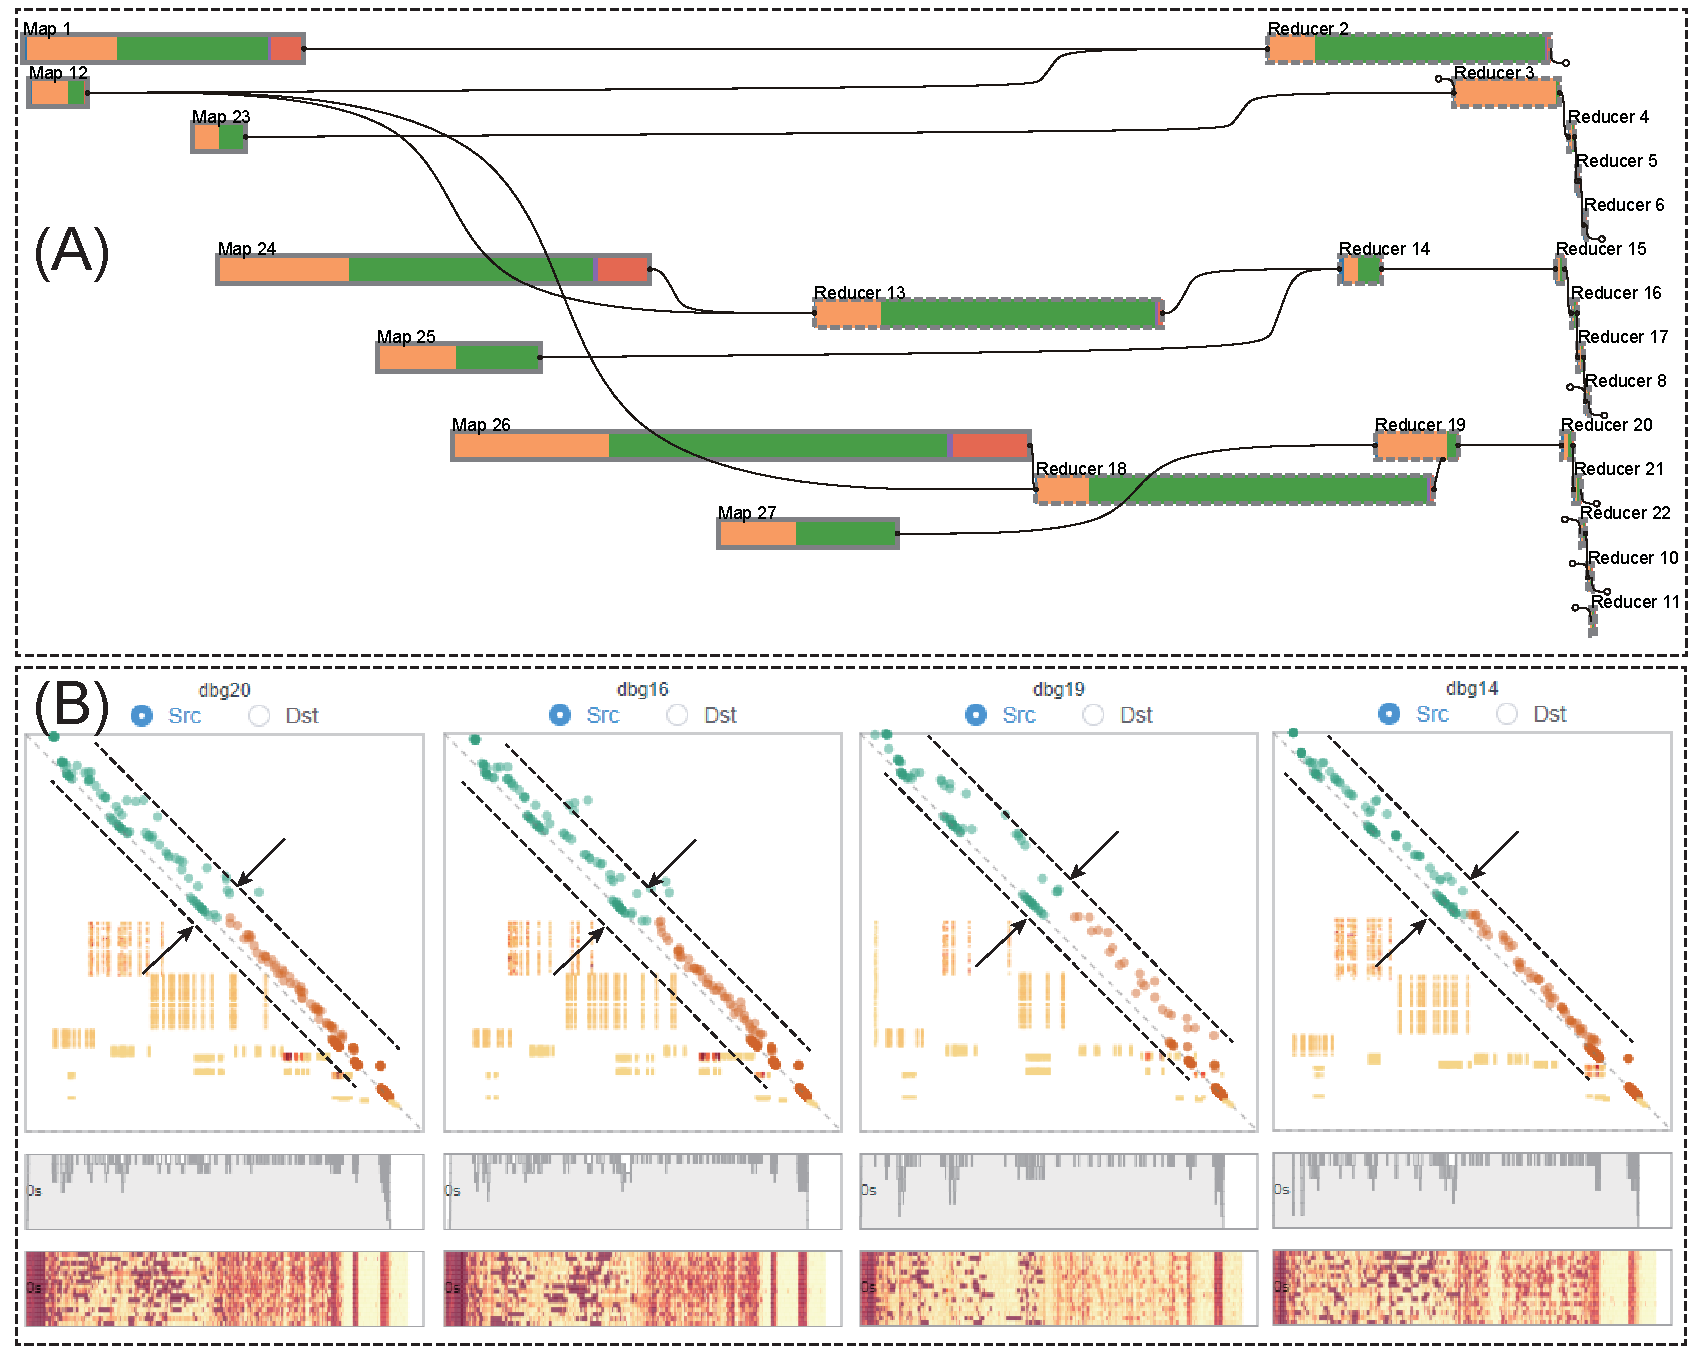
\includegraphics[width=0.45\textwidth]{figures/case_study/CaseStudy1.pdf}
	\vspace{-3mm}
	\caption{Re-execute the query after removing a unhealthy node and stop the CPU-bound programs.}
	\label{fig:casestudy1}
	\vspace{-3mm}
\end{figure}


To address this problem, we directly remove the node dbg18, stop the other programs run on server dbg19 and re-execute the same query. The query is finished with 200s. In the progress view, we find the duration of both vertex Map1 and Map24 are greatly reduced shown as Figure~\ref{fig:casestudy1}(A). We also find that in the distribution view, all the tasks are distributed close to the diagonal line indicating that they are all executed within the small time range Figure~\ref{fig:casestudy1}(B). Moreover, the CPU performance view shows that all the CPUs on different server have the balanced performance. 

\subsubsection{Diagnose the task failure}



\begin{figure*}
	\vspace{2mm}
	\centering
	\small
	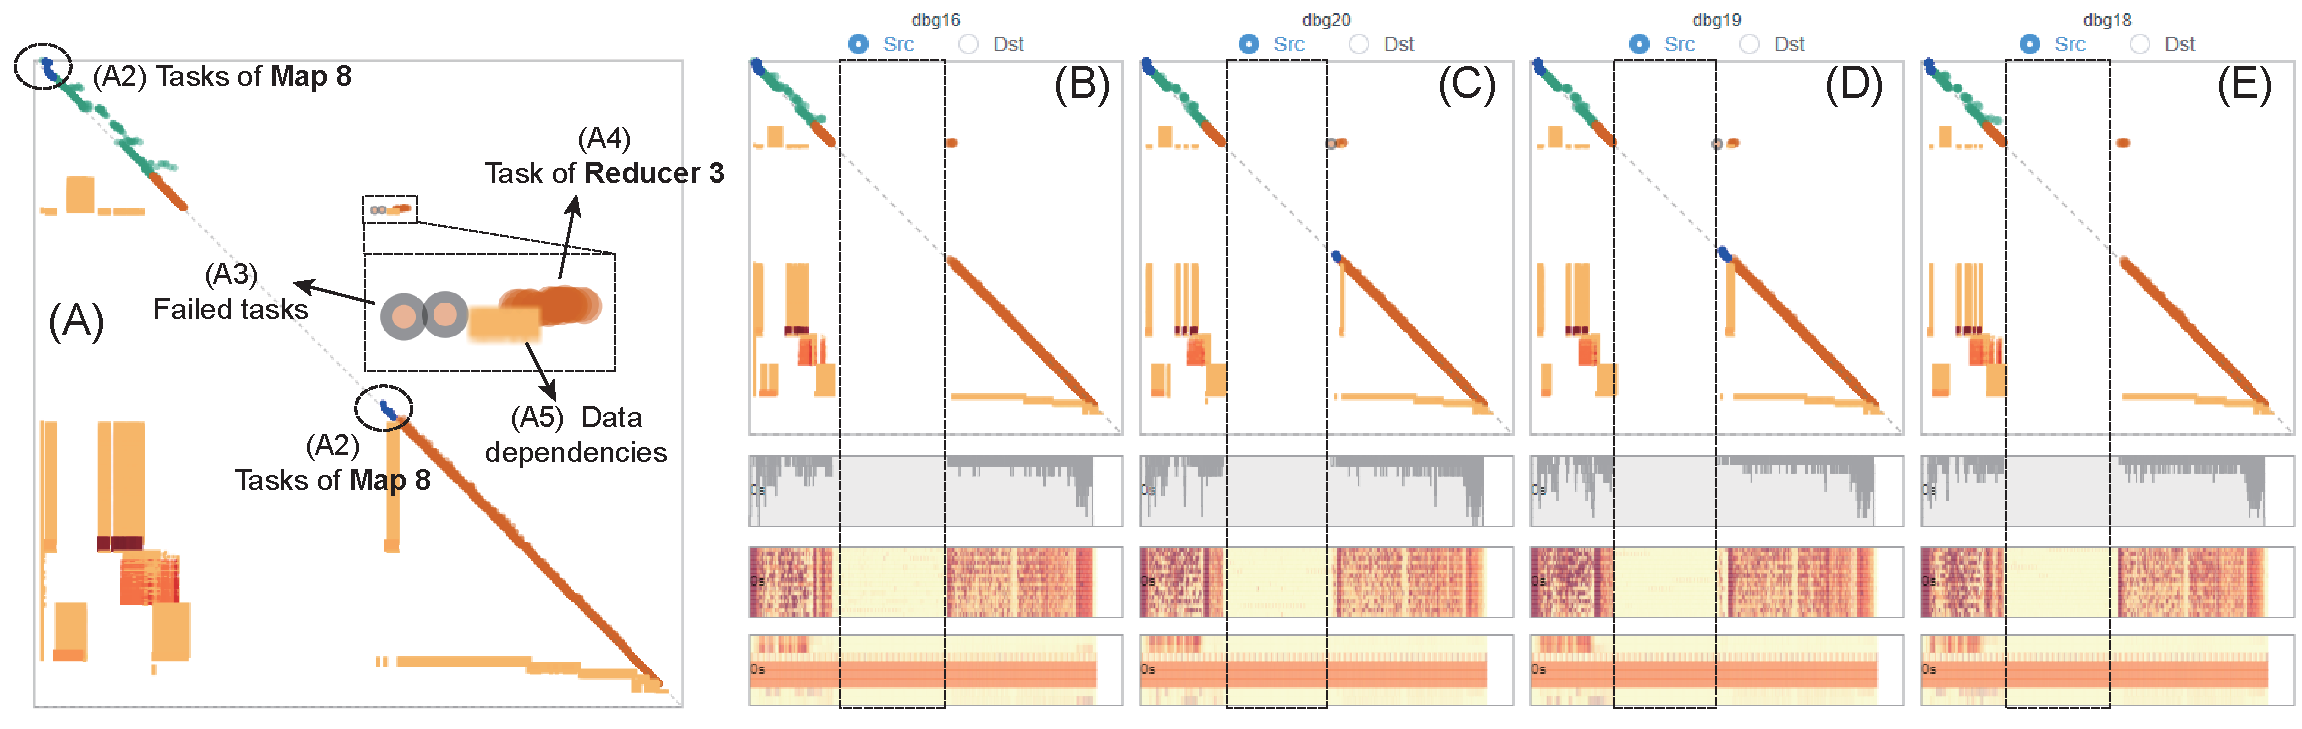
\includegraphics[width=2\columnwidth]{figures/case_study/CaseStudy2.pdf}  

	%\vspace{-3mm}
	\caption{Analyze the task failure.} 
	\label{fig:casestudy2}

\end{figure*}


The second case runs on the cluster with four nodes. As show by the summary view,  we notice that there are two tasks failed during the execution. The expert wants to know how why these tasks are failed. By observing the performance view, we notice during the execution of the failed tasks, the all the machine run the maximum number of tasks but the usage of their CPU, memory and network are not fully used, which indicating these tasks take the quota of the works but do nothing. but cannot finished until two tasks are abandoned.
***

\subsubsection{Understand the data skew}

\begin{figure}[t]
	\centering
	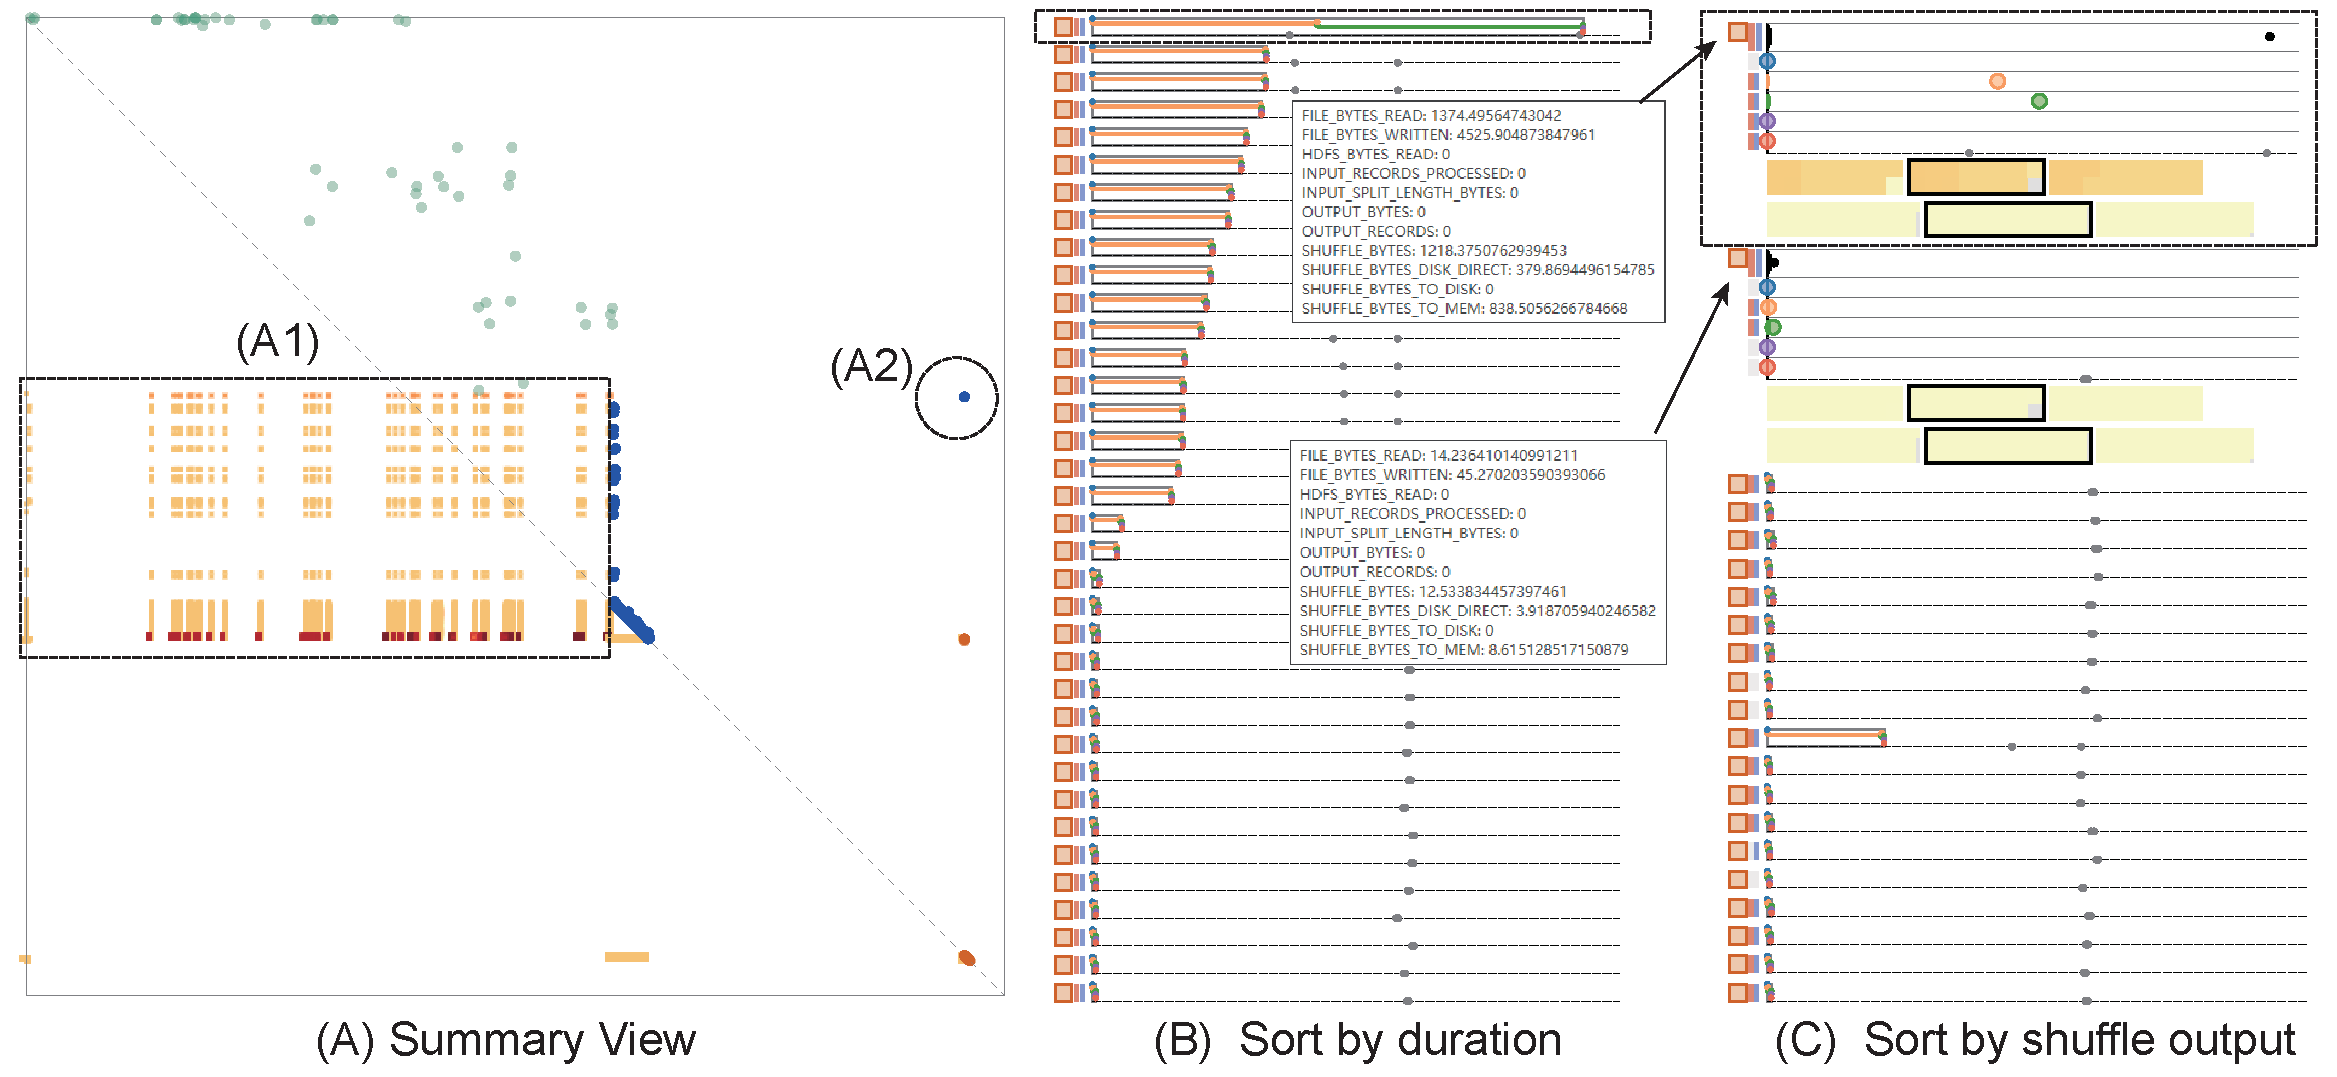
\includegraphics[width=0.45\textwidth]{figures/case_study/CaseStudy3.pdf}
	\vspace{-3mm}
	\caption{Detect the data skew.}
	\label{fig:casestudy3}
	\vspace{-3mm}
\end{figure}
